\chapter{Géométrie vectorielle}
\label{chapter:Fr_02-vectors}
 
Une grande partie du contenu de ce chapitre est sans doute une revue de la géométrie vectorielle déjà étudiée au lycée, mais cela nous permettra de préparer le terrain 
 pour les chapitres à venir.



\section{Vecteurs de \texorpdfstring{$\R^n$}{Rn}}

Le mot \stress{vecteur} vient du latin \textit{vehere} qui signifie porter, transmettre. De façon abstraite, lorsque l'on dessine un vecteur avec une flèche, on peut se dire en quelque sorte que le vecteur nous emmène d'un bout à l'autre de la flèche, dans la direction indiquée par la flèche.  Par exemple, on utilise les vecteurs en physique pour indiquer l'intensité et la direction d'une force.


Dans ce qui suit, nous ferons appel à notre compréhension de la géométrie et de l'algèbre en
dimensions 2 et 3 pour généraliser les idées aux dimensions supérieures.

\begin{center}
\begin{tabular}{ll}
Algèbre & Géométrie \\
\hline
$\R$: nombres réels, \defn{scalaires} & droite réelle\\ 
$\R^2 = \{(x,y) | x,y\in\R\}$, vecteurs $\uu = (x,y)$ & plan \\ 
$\R^3 = \{(x,y,z) | x,y,z\in\R\}$, vecteurs $\uu = (x,y,z)$ & espace tridimensionnel\\
\quad\quad\vdots & \\
(pourquoi ne pas continuer ?) & \\
\quad\quad\vdots & \\
$\R^4 = \{(x_1,x_2,x_3,x_4) | x_i \in \R\}$, vecteurs $\xx = (x_1,x_2,x_3,x_4)$ & \\ 
Hamilton (1843) : extension de $\C$ aux \defn{hamiltoniens} & \defn{espace temps}\\ 
& \\
$n \in \Z$, $n>0$ : $\R^n = \{ (x_1, x_2, \cdots,x_n) | x_i \in \R\}$, &\\
vecteurs $\xx = (x_1, \cdots, x_n)$ & espace de dimension $n$
\end{tabular}
\end{center}

\paragraph{\bf Notations:}  Voici les différentes notations équivalentes pour écrire un vecteur $\xx$ de $\R^4$ par exemple. Nous les utiliserons de manière interchangeable :
\begin{itemize}
\item $\xx = (1,2,3,4)$;
\item $\xx = \mat{1\\2\\3\\4}$;
\item $\xx = \mat{1\;&2\;&3\;&4}^T$, où l'exposant T signifie qu'on prendre la
\defn{transposée} du vecteur ligne.  (\emph{Transposer}\index{transposer} signifie par définition transformer les lignes en colonnes et \textit{vice versa} les colonnes en lignes.)
\end{itemize}
La notation verticale (également appelée \defn{forme matricielle}) est la plus facile à lire, mais la première notation est plus facile
à écrire.
(La notation verticale vient de la multiplication matricielle que nous aborderons plus tard).

\section{Manipulation des vecteurs de \texorpdfstring{$\R^n$}{Rn}}  

L'algèbre des vecteurs de $\R^n$ se déduit directement de celle qu'on connaît déjà dans $\R^2$ et $\R^3$ : 
\begin{itemize}
\item égalité: $(x_1,\cdots, x_n) = (y_1,\cdots, y_n) \,\Longleftrightarrow\,  (x_i=y_i$ pour tout $i \in \{1,\cdots,n\})$.  En particulier on a toujours $(x_1,\cdots,x_n) \neq (y_1,\cdots, y_m)$ lorsque $n \neq m$;

\item addition : $(x_1,\cdots,x_n) + (y_1,\cdots, y_n) = (x_1+y_1, \cdots, x_n+y_n)$;
\item vecteur nul : $\zero = (0,0,\cdots, 0) \in \R^n$;
\item inverse additif ou oppos\'e : si $\xx = (x_1,\cdots,x_n)$, alors $-\xx = (-x_1,\cdots,-x_n)$;
\item multiplication {\bf par un scalaire} : soit $c\in \R$ un scalaire, alors
$c\,(x_1,\cdots,x_n) = (c\,x_1,\cdots,c\,x_n)$.
\end{itemize}
Notez que nous n'avons aucun moyen de \stress{multiplier} deux vecteurs; néanmoins, ce qui s'en rapproche le plus est sans doute le \stress{produit scalaire}, qui multiplie deux vecteurs en un certain sens et renvoie un scalaire, c'est-à-dire un nombre de $\R$. Dans le cas de la dimension $3$, \textit{i.e.} dans $\R^3$, il y a également le \stress{produit vectoriel}, qui multiplie deux vecteurs en un certains sens et renvoie un autre vecteur.\footnote{Il existe aussi des moyens de généraliser ce produit vectoriel de $\R^3$ à $\R^n$ pour $n$ quelconque, mais la particularité est que le résultat du produit n'appartient plus à  $\R^n$... Cherchez sur le web « algèbre extérieure ».}
 Il y a également une méthode pour pour construire des «~produits multiples~» de $n-1$  vecteurs de $\R^n$ et d'obtenir une réponse aussi dans $\R^n$. Quoi qu'il en soit, une fois que nous aurons vu le {\it déterminant }, vous comprendrez plus aisément le sens de la définition du produit vectoriel.

Il existe une interprétation géométrique de chacune des règles algébriques données ci-dessus. Vous pouvez même les dessiner dimension $2$ (voire aussi en dimension $3$ si vous dessinez bien !) :

\begin{itemize}
\item égalité : deux vecteurs sont égaux ssi ils ont la même longueur et la même direction;
\item addition : règle du parallélogramme;
\item vecteur nul : le vecteur de longueur nulle;
\item oppos\'e : la même flèche mais avec tête et queue échangées;
\item multiplication par un scalaire $c\in\R$ : vecteur dont la longueur est $\vert c \vert$ fois celle du vecteur de départ et dont la direction est inversée si $c<0$. Donc deux vecteurs sont \emph{parallèles} si et seulement si 
on peut passer de l'un à l'autre en faisant simplement une multiplication par un scalaire.
\end{itemize}

\section{Combinaisons linéaires (concept important !)}
Les seules opérations sur les vecteurs que nous utiliserons pour l'instant sont : l'addition et la multiplication par un scalaire.
Nous allons nous intéresser à la question suivante.  
Si l'on a $m$ vecteurs de $\R^n$, disons $\uu_1$, ${\uu_2}$, $\cdots$, ${\uu_m}$, et que l'on s'autorise à les dilater et à les sommer, peut-on obtenir un nouveau vecteur qui ne figure pas parmi ces $m$ vecteurs
 ?

La réponse est OUI. Donnons un exemple :  considérons un vecteur ${\uu_1}$ parallèle à la rue Bank, pointant vers le nord,
et un vecteur ${\uu_2}$  parallèle à l'avenue Laurier, pointant vers l'est. Alors, en partant de l'université, on peut se rendre n'importe où dans le centre-ville en 
combinant des déplacements vers le nord grâce à ${\uu_1}$ (ou vers le sud grâce à son opposé), et vers l'est grâce à ${\uu_2}$ (ou vers l'ouest grâce à son
opposé). En revanche, on ne peut pas aller sous terre ni
dans les airs car on n'a pas de vecteur qui nous permet de changer notre hauteur.  En fait, on est limité à des déplacements dans le plan du sol, on ne peut ni aller plus haut, ni aller plus bas.

Algébriquement, tout cela se résume en la définition suivante :


\begin{definition} \index{combinaison linéaire}
Étant donnés des scalaires $k_1, k_2, \cdots, k_m \in \R$ et des vecteurs ${\uu_1}, {\uu_2}, \cdots, {\uu_m}\in \R^n$, on définit le vecteur 
$$
k_1\,{\uu_1} + k_2\,{\uu_2} + \cdots + k_m\,{\uu_m} \in \R^n,
$$
et on l'appelle \emph{combinaison linéaire} de ${\uu_1},{\uu_2},\cdots,{\uu_m}$ avec \emph{coefficients} (ou \emph{poids}) $k_1, k_2, \cdots, k_m$.
\end{definition}

\begin{myexample}
Soit ${\uu_1} = (1,2,3)$ et ${\uu_2} = (1,0,0)$.  

Alors $\xx = (17,4,6)$ est une combinaison linéaire de ${\uu_1}$ et de ${\uu_2}$ car
$$
\mat{17\\4\\6} = 2 \mat{1\\2\\3} + 15 \mat{1\\0\\0}.
$$
Par contre $\yy = (0,1,0)$ \emph{n'est pas} une combinaison linéaire de
${\uu_1}$ et ${\uu_2}$. En effet, l'équation
\begin{equation} \label{E:1}
\mat{0\\1\\0} = a \mat{1\\2\\3} + b\mat{1\\0\\0}
\end{equation}
impliquerait 
\begin{align*}
\mat{0\\1\\0} &= \mat{a\\2a\\3a} + \mat{b\\0\\0}\\
&= \mat{a+b\\2a \\3a}
\end{align*}
et donc
$$
0 = a+b, \quad 1 = 2a, \quad \text{et} \quad 0 = 3a,
$$ 
ce qui est absurde car les deux dernières égalités sont contradictoires : $a=\frac12$ et $a=0$... D'o\`u
il ne peut y avoir de solution à l'équation \eqref{E:1}, et ainsi $\yy$
ne peut pas être une combinaison linéaire de ${\uu_1}$ et ${\uu_2}$.
\end{myexample}


\section{Propriétés de l'addition vectorielle et de la multiplication par un scalaire}


On a vu que l'addition de deux vecteurs $\uu+\vv$ est similaire dans $\R^n$ à celle que l'on connaissait dans $\R^2$, et de même pour la multiplication par un scalaire $c\,\uu$.
Il en découle donc que toutes les propriétés algébriques dans $\R^2$ de l'addition et de la multiplication par un scalaire restent valables dans $\R^n$.  En d'autres termes, si l'on se donne des vecteurs $\uu,\vv,\ww\in\R^n$ et des scalaires $c,c' \in \R$, on a:
\begin{itemize}
\item $\uu+\zero = \uu$;
\item $\uu + (-\uu) = \zero$;
\item $(\uu + \vv) + \ww = \uu + (\vv+\ww)$;

\item $\uu+\vv = \vv+\uu$;
\item $c\,(\uu+\vv) = c\,\uu + c\,\vv$;
\item $(c+c')\,\uu = c\,\uu + c'\,\uu$;
\item $(cc')\,\uu = c\,(c'\,\uu)$;
\item $1\,\uu = \uu$.
\end{itemize}
Gardez ces propriétés en tête, car elles sont la clé pour la généralisation
aux espaces vectoriels encore plus généraux que $\R^n$.

\section{Plus de géométrie : le produit scalaire dans  \texorpdfstring{$\R^n$}{Rn}}

Le \defn{produit scalaire} nous donne
un moyen algébrique d'étudier certaines propriétés géométriques intéressantes, comme
la longueur d'un vecteur ou l'angle entre deux vecteurs.

Rappelons la définition du produit scalaire dans $\R^3$.
Soient $\uu = (x_1,x_2,x_3)$ et $\vv = (y_1,y_2,y_3)$ deux vecteurs de
$\R^3$.  Alors leur produit scalaire est définit comme :
$$
\uu \cdot \vv = x_1\,y_1 + x_2\,y_2 + x_3\,y_3.
$$
Notez que le résultat est un scalaire, c'est-à-dire un nombre réel.

Une fois que l'on a introduit le produit scalaire, on peut définir:
\begin{itemize}
\item la \emph{longueur} ou \emph{norme} de $\uu$ : $\Vert \uu \Vert = \sqrt{x_1^2+x_2^2+ x_3^2} = \sqrt{\uu \cdot \uu}$;
\item la \emph{distance entre $\uu$ et $\vv$} : $\Vert \uu - \vv \Vert$.
\end{itemize}
On peut visualiser ceci en dessinant un parallélépipède rectangle dont la diagonale principale est $\uu$:
on remarque alors que la longueur de la diagonale principale est donnée par la racine carrée
de la somme des carrés des longueurs des côtés (ceci est vrai par applications répétées du théorème de Pythagore).

Généralisons donc cela à $\R^n$!

\begin{definition}
Soient $\uu = (x_1,\ldots,x_n)$ et $\vv = (y_1,\ldots,y_n)$ des vecteurs
de $\R^n$.  Alors leur \defn{produit scalaire} est défini comme étant : 
$$
\uu \cdot \vv = x_1\,y_1 + \cdots + x_n\,y_n,
$$
et la \defn{norme} de $\uu$ est définie comme étant :
$$
\Vert \uu \Vert = \sqrt{\uu \cdot \uu} = \sqrt{x_1^2+\cdots+x_n^2}\,.
$$
L'espace $\R^n$  muni du produit scalaire est parfois décrit comme un \defn{espace euclidien  de dimension $n$}.
\footnote{Contrairement à l'« espace-temps de Minkowski » par exemple, où les « longueurs » des vecteurs peuvent être imaginaires ! Cherchez sur le web « espace de Minkowski ».}
\end{definition}


\begin{myexample}
Soient $\uu = (1,2,-1,0,1)$ et $\vv = (1,3,2,1,1)$.  Alors
$$
\uu \cdot \vv = 1+6-2+0+1 = 6
$$
et
$\Vert \vv \Vert = \sqrt{1+9+4+1+1} = \sqrt{16}=4$.
\end{myexample}

Notez que pour tout vecteur $\uu \in \R^n$ :
$$
\Vert \uu \Vert = 0 \Leftrightarrow \uu = \zero
$$
(parce que la norme est toujours la somme de carrés des composantes réels, et donc
n'est jamais nulle, sauf si chaque composante l'est).

\section{Orthogonalité}
\label{section : orthogonalite}

Rappelons que dans $\R^2$ et $\R^3$, on a l'équivalence :
$$
\uu \cdot \vv = 0 ~\Longleftrightarrow \textrm{$\uu$ et $\vv$ sont «~orthogonaux~» (ou «~perpendiculaires~»).}
$$

\begin{definition}
Soient $\uu,\vv \in \R^n$.  On dit que $\uu$ et $\vv$ sont
\emph{orthogonaux}\index{orthogonaux, vecteurs} si $\uu \cdot \vv = 0$.
\end{definition}

\begin{myexample}
Les vecteurs $(1,2,-2,1)$ et $(4,1,3,0)$ de $\R^4$ sont orthogonaux puisque
$$
\mat{1\\2\\ -2\\1} \cdot \mat{4\\1\\3\\0} = 4+2-6+0 = 0\,.
$$
\vglue -.5cm
\end{myexample}

\section{Angles entre vecteurs dans \texorpdfstring{$\R^n$}{Rn}}

Dire que deux vecteurs sont orthogonaux dans $\R^2$ ou $\R^3$ signifie aussi qu'ils se croisent en un angle droit (soit $90^\circ$).  En fait, nous pouvons déterminer l'angle entre deux vecteurs de $\R^2$ ou de $\R^3$ grâce au produit scalaire. D'o\`u la question: 
peut-on généraliser ceci?  Nous avons besoin de la formule suivante:


\begin{theorem} [Inégalité de Cauchy-Schwarz]
Si $\uu,\vv \in \R^n$, alors 
$$
\vert \uu \cdot \vv \vert \leq \Vert \uu \Vert \; \Vert \vv \Vert\,.
$$
\end{theorem}

La preuve\footnote{Pour $x\in\R$, considérez la fonction quadratique $q(x)=\|u+ x v\|^2$. Écrivez le côté droit comme $(u+ x v)\cdot (u+ x v)$, développez pour obtenir un polynôme de degré $2$ et calculez le discriminant «~$b^2-4ac$~». Le discriminant doit satisfaire $b^2-4ac\le 0$ puisque $q(x)\ge 0$ pour tout $x$ implique qu'on ne peut pas avoir deux racines réelles distinctes. En simplifiant, on obtient l'inégalité désirée.} est simple.

En appliquant ceci à $\Vert \uu + \vv \Vert^2 = (\uu + \vv)\cdot(\uu+\vv)$
on obtient
$$
\Vert \uu + \vv \Vert \leq \Vert \uu \Vert + \Vert \vv \Vert,
$$
et on retrouve la fameuse \defn{inégalité triangulaire}. Notez qu'elle ressemble beaucoup à celle annoncée pour $\C$
dans notre premier chapitre.

\begin{definition}
Si $\uu,\vv \in \R^n$ et $\uu,\vv \neq \zero$, alors l'angle
$\theta$ entre $\uu$ et $\vv$ est défini comme étant l'unique nombre
$\theta\in\R$ satisfaisant :
\begin{itemize}
\item $\displaystyle \cos \theta = \frac{\uu \cdot \vv}{\Vert \uu \Vert\; \Vert \vv \Vert}$;
\item $0 \leq \theta \leq \pi$.
\end{itemize}
(La première condition est une conséquence de l'inégalité de Cauchy-Schwarz, puisque cette inégalité implique que le membre de droite est toujours compris entre $-1$ et $1$. La deuxième condition garantit l'unicité de $\theta$. )
\end{definition}

\begin{myexample}
L'angle $\theta$ formé par $\uu = (0,0,3,4,5)$ et $\vv = (-1,1,-1,1,2)$ doit satisfaire :
$$
\cos(\theta) = \frac{\uu \cdot \vv}{\Vert \uu \Vert\; \Vert \vv \Vert}
= \frac{11}{\sqrt{50}\sqrt{8}} = \frac{11}{20},
$$
donc on trouve $\theta = \arccos(11/20)$.\footnote{\`A l'aide d'une calculatrice - ce dont vous n'aurez jamais besoin dans ce cours, on arrive à $\theta \simeq 0.988432\simeq56.6^\circ$.}
\end{myexample}

Énonçons deux remarques intéressantes :
\begin{itemize}
\item Deux vecteurs non nuls $\uu$ et $\vv$ sont orthogonaux ssi l'angle entre eux est $\frac{\pi}2$ (ou $90^\circ$).  Comme $\cos(\frac{\pi}2) = 0$, notre formule ci-dessus nous dit que
le numérateur $\uu \cdot \vv$ doit être nul.  C'est de là que vient en fait la
condition d'orthogonalité $\uu \cdot \vv=0$ de la section \ref{section : orthogonalite}.
\item Deux vecteurs $\uu$ et $\vv$ sont parallèles ssi l'angle entre eux est soit $0^\circ$ soit $\pi$.  Notons que comme $\cos(0) = 1$ et
$\cos(\pi) = -1$ , notre formule ci-dessus donne $\uu \cdot \vv = \pm \Vert \uu \Vert\; \Vert \vv \Vert$, et le produit scalaire atteint donc sa valeur maximale dans les deux cas (en terme de valeur absolue).
\end{itemize}




\section{Projection orthogonale sur une droite dans \texorpdfstring{$\R^n$}{Rn}}
\label{section : projection orthogonale sur une droite dans Rn}
 
L'idée de la 
projection orthogonale est la suivante : étant donnés deux vecteurs non nuls $\uu$ et $\vv$,
 la \defn{projection de $\vv$ sur $\uu$}, notée

  
$$
 \proj_{\uu}(\vv),
$$ 
est l'unique vecteur satisfaisant les deux conditions suivantes :
\begin{itemize}\label{propOrthogProj}
\item $\proj_{\uu}(\vv)$ est parallèle à  
$\uu$ (c'est donc un multiple scalaire de $\uu$);
\item $\vv - \proj_{\uu}(\vv)$ est orthogonal à $\uu$ (c'est donc un vecteur qui donne un produit scalaire nul avec $\uu$).
\end{itemize}
 
\begin{figure}
\begin{center}
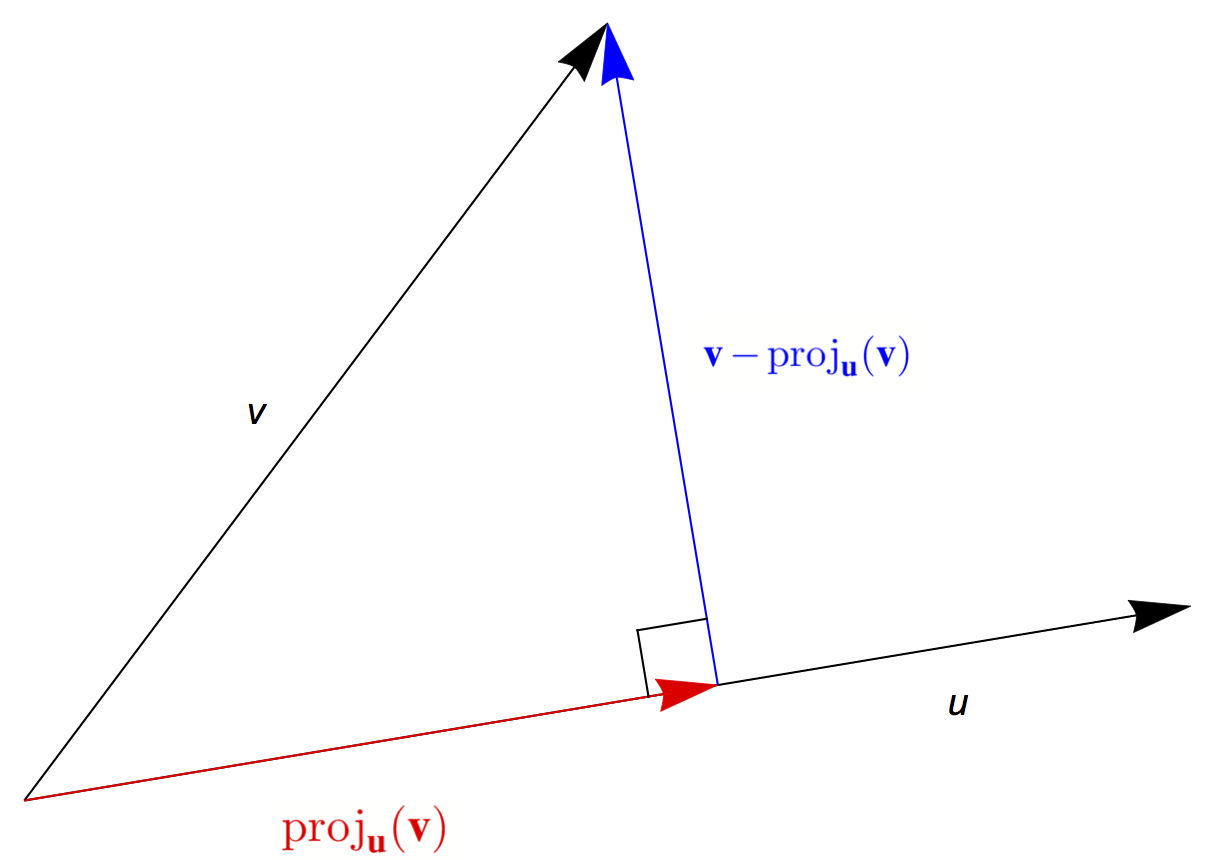
\includegraphics[scale=.4]{decomp.jpg}~\\[1cm]
\end{center}
\caption{Projection orthogonale de $\vv$ sur $\uu$.}\label{orthoprojonvector}
\end{figure}
En particulier, ceci permet de \stress{décomposer} n'importer quel vecteur  $\vv$ comme la somme suivante :
$$
\vv = (\proj_{\uu}(\vv))+ (\vv-\proj_{\uu}(\vv)),
$$
dont le premier terme est un vecteur parallèle à $\uu$ et le second est un vecteur perpendiculaire à $\uu$,
comme représentés dans notre figure \ref{orthoprojonvector}.

Alors comment calcule-t-on $\proj_{\uu}(\vv)$ ?  Ceci s'avère en fait facile.
En utilisant la trigonométrie, ou en résolvant directement les deux conditions ci-dessus, on aboutit à :
$$
\proj_{\uu}(\vv) = \frac{\vv \cdot \uu}{\Vert \uu \Vert^2} \,\uu.
$$\label{projR3}
(Attention : le quotient est juste un scalaire.  Pour s'en souvenir :
si vous projettez $\vv$ sur $\uu$, le résultat est toujours un vecteur qui est un multiple scalaire du vecteur $\uu$. Notez que c'est le même $\uu$ qui apparaît aussi dans la norme au dénominateur).

\begin{myexample}
Soient $\uu = (1,0,0)$ et $\vv = (2,3,4)$.  Écrivons $\vv$ comme une somme
de deux vecteurs, l'un parallèle à $\uu$ et l'autre orthogonal à $\uu$.
(Bien sûr, c'est toujours possible de «~deviner à tâtons~» la réponse, mais voyons plutôt ce que donne la formule).
On calcule
$$
\proj_{\uu}(\vv) = \frac{\vv \cdot \uu}{\Vert \uu \Vert^2} \,\uu
= \frac{2+0+0}{1^2+0^2+0^2}\mat{1\\0\\0} = \mat{2\\0\\0}
$$
et $\vv - \proj_{\uu}(\vv) = (2,3,4)-(2,0,0) = (0,3,4)$. Notre
décomposition est alors
$$
\vv = \mat{2\\3\\4} = \mat{2\\0\\0}+\mat{0\\3\\4}
$$
et il est clair qu'on a obtenu le bon résultat : le premier vecteur est parallèle à $\uu$ tandis que 
le second lui est orthogonal. Notez que c'est la seule
paire de vecteurs à satisfaire ceci.
\end{myexample}

\begin{myexample} 
Soient $\uu = (1,1)$ et $\vv = (2,3)$.  Alors
$$
\proj_{\uu}(\vv) = \frac{\vv \cdot \uu}{\Vert \uu \Vert^2} \uu
= \frac{2+3}{1^2+1^2}\mat{1\\1} = \mat{5/2\\5/2}
$$
est la projection de $(2,3)$ sur $(1,1)$.
\end{myexample}

Dans la vie de tous les jours, la projection orthogonale est utilisée dans le système UMTS (système universel de télécommunications mobiles) pour corriger les perturbations et les erreurs dans les signaux, et pour produire des communications plus fiables.

Remarque : une autre façon d'interpr\'eter la projection orthogonale est de dire que
nous trouvons le point le plus proche de $\vv$ sur la droite passant par l'origine et dirigée par $\uu$.  
Notre prochain objectif est donc de discuter de droites et de plans.


